\documentclass[a4paper, 11pt, draft]{report}

\usepackage[utf8]{inputenc} % Texte en utf-8
\usepackage{aeguill}
\usepackage[francais]{babel} % Typographie française
\usepackage[pdftex, hypertexnames=false, colorlinks=true, final]{hyperref}
\usepackage[final]{graphicx}
\usepackage{url} % Gestion des URLs
\usepackage{geometry}
\usepackage{fancyhdr}
\usepackage[Lenny]{fncychap}

% Marges à gauche et à droite de 3cm
\geometry{margin=3cm}

% Utilisation des headers et footers personnalisés de fancyhdr
\pagestyle{fancy}

% Images dans le dossier ./images/
\graphicspath{{./images/}}

% Gestion des métadonnées étranges à rendre visibles au rendu
\newcommand\docname{PMPv0.2 (Draft)}
\newcommand\docauthor{Guillaume Bouchard}
\newcommand\docstatus{LIVRABLE} % EN COURS, ATTENTE, VALIDE ou LIVRABLE

% Numérotation mieux ; pour l'instant, on garde le défaut
% \renewcommand\thechapter{\Alph{chapter}}
% \renewcommand\thesection{\Roman{section}}
% \renewcommand\thesubsection{\arabic{subsection}}
% \renewcommand\thesubsubsection{\alph{subsubsection}}

% Format de citation de références standard, marche avec quasiment tout
\newcommand\fullref[1]{\ref{#1}, page \pageref{#1}}

% En-têtes et pieds de page
\lhead{\docname}
\rhead{}
\lfoot{Auteur : H4213}
\cfoot{}
\rfoot{\thepage}

% Titre du document maître
\title{\textbf{COPEVUE}\\
\rule{\textwidth}{1pt}{}\\
\Huge{\textsc{Plan management projet}}}
\author{\docauthor{}}
\date{\docname{} --- \today{} (\docstatus{})}



\begin{document}

\maketitle

\tableofcontents

\pagebreak


\chapter{Introduction}

\section{Présentation du document}

Ce document a pour but de donner une vision globale de la gestion du projet de \emph{système de surveillance à distance de sites isolés} sur différents points, aussi bien organisationnels, temporels, activité et produits.

Il existe dans le but de servir de document contractuel pour renseigner le comité de direction du projet, au sein de la COPEVUE, et ainsi permettre à celui-ci de valider les dispositions prises par le chef de projet pour la bonne marche de ce projet.


\section{Statut du document}

Ce document est un Draft, c'est à dire un document de travail non finalisé et doit donc être traité en tant que tel.

\section{Cadre du PMP}

Ce document est la suite logique du dossier d'initialisation réalisé pour l'étude préalable en vue de répondre à l'appel d'offre de la COPEVUE.

Comme ce document doit couvrir l'organisation de tout le projet, depuis l'étude approfondie, en passant par la conception, la réalisation et la mise en oeuvre du système, il se doit d'être plus conséquent.


\section{Documents liés}


Le document qui sert de base à ce plan de management de projet est le dossier d'initialisation réalisé lors de l'étude préalable. Celui-ci est fourni en annexe de ce document.

Ce document est applicable à tous les produits et acteurs du projet quels que soient leurs types. En effet il couvre l'étendue du projet et doit servir de référence à tous les acteurs du projet, de la maîtrise d'œuvre à la maîtrise d'ouvrage.

On pourra se référer aux documents \emph{Manuel du CdC} et au guide d'évaluation des charges distribué en début de projet.


\subsection{Rappel du contexte}

Il existe aujourd'hui de nombreux sites isolés et/ou difficiles d'accès qui nécessitent une surveillance et parfois des actions à distance. Ces sites se situent dans des espaces très différents tels que les citernes placées dans les forêts escarpées du pourtour méditerranéen, les réservoirs utilisés pour l'autonomie des chantiers dans le grand Nord mais aussi les personnes âgées qui se retrouvent souvent isolées.

Actuellement tous les contrôles et actions sont réalisés par un opérateur qui doit se déplacer sur le site. Il n'y a donc que très peu de réactivité, on ne peut pas avoir un suivi fin des évolutions et des problèmes graves -- par exemple la fuite d'un réservoir -- ne peuvent pas être traités rapidement.

Le but principal du ce projet est donc d'optimiser cette chaîne de traitement en limitant le nombre d'interventions humaines sur site grâce aux traitement à distance et en facilitant l'organisation et la gestion de ces interventions lorsqu'elles auront lieu.


\chapter{Organisation du projet}

\section{Organisation des structures décisionnelles}

Il existe trois acteurs principaux dans ce projet qui sont listés par ordre de déférence.

\subsection{Le comité de pilotage}

C'est lui qui a lancé l'appel d'offre et qui attend le résultat. Il s'agit du client que notre bureau d'étude va tenter de satisfaire. C'est lui qui fixe le cadre général du projet (le résultat attendu et la répartition temporelle).

\subsection{Le groupe d'étude principal}

Il s'agit de notre groupe d'étude. C'est lui qui prend en charge le projet dans son organisation et dans sa conception globale.

\subsection{Les différents intervenants}

Il s'agit de toutes les sociétés externes qui pourrait prendre part à ce projet, en répondant par exemple aux appels d'offres lancés par notre groupe d'étude pour la réalisation des sous projets.

 Tout cela est résume dans la figure \ref{glops2}


\begin{figure}[htbp]
\begin{center}
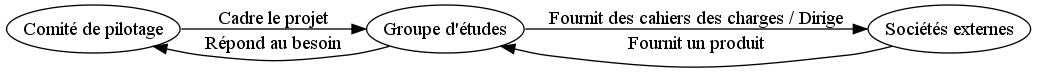
\includegraphics[width=\textwidth]{relations.png}
\caption{Relations entre les acteurs\label{glops2}}
\end{center}
\end{figure}
\section{Organisation du développement}

Lors d'une première phase, bien détaillée dans le dossier d'initialisation fourni en annexe, le groupe d'étude aura ciblé le projet et réalisé sa conception globale. De plus, pour chaque sous-projet défini dans la suite de ce document, il sera fait appel à des sociétés externes pour sa réalisation.


\subsection{Réalisation du cahier des charges}


Notre groupe d'étude réalise les cahiers des charges de chaque sous projet. En annexe de ces cahiers des charges se trouve un dossier d'interface entre les sous-projets.

Ces deux documents doivent permettre à toute société externe de réaliser un sous projet en répondant au besoin et s'intégrant parfaitement avec les autres sous-projets.

Chaque cahier des charges se voit attribuer un responsable au sein du groupe d'étude qui deviendra l'interlocuteur avec les sociétés externes en charge des sous-projets.

\subsection{Appel d'offres}

Un appel d'offres par cahier des charges est lancé sur le marché. En fonction de la complexité -- aussi bien technique que temporelle -- du sous projet, celle-ci étant évaluée dans les cahiers des charges respectifs, il est donné une date limite de réponse aux appels d'offres aux sociétés intéressées.

A la date convenue, celles-ci présenteront leurs propositions au bureau d'étude qui fera son choix parmi les différentes propositions.

Si possible, dans le cas où une même société propose une réponse pour plusieurs cahiers des charges, et que celle-ci est compétente, elle sera choisie ce qui facilitera grandement la communication entre sous-projets et réduira le nombre d'acteurs externes à gérer. De plus cela peut aussi amener à une diminution des coûts.

Pour certains sous projets, si le responsable de celui-ci le juge utile, plusieurs réponses, venant de sociétés différentes seront acceptées et les résultats fournis seront mis en concurrence à la fin. Ce genre de cas doit être extrêmement rare du fait de la complexité qu'il impliquera et des surcoûts engendrés, cependant cela peut être nécessaire dans le cas de sous-projets très critiques.


\subsection{Conception et réalisation}

La société gérant le sous projet a carte blanche pour sa méthode de développement et de conception -- si elle le désire elle peut utiliser des méthodes agiles par exemple -- cependant elle doit présenter des revues périodiques d'avancement, dont la période sera définie par le responsable du projet et ne devra jamais être supérieure à 6 semaines.


Les rendus doivent suivre une politique de qualité très stricte, définie par le responsable qualité du groupe d'étude. Par exemple dans le cas de développement logiciel, la documentation fournie doit être la plus exhaustive possible et tous les tests réalisés lors de la création du logiciel doivent pouvoir être rejoués.


\subsection{Intégration et recette}

Le sous projet une fois terminé subira des tests d'intégration et de recette pour vérifier sa conformité au cahier des charges. A ce moment il est possible que le produit retourne à la société pour subir différentes modifications en cas de non conformité aux cahiers des charges, problèmes d'intégration ou modifications des besoins.

Tout cela est résumé dans la figure \ref{glops}


\begin{figure}[htbp]
\begin{center}
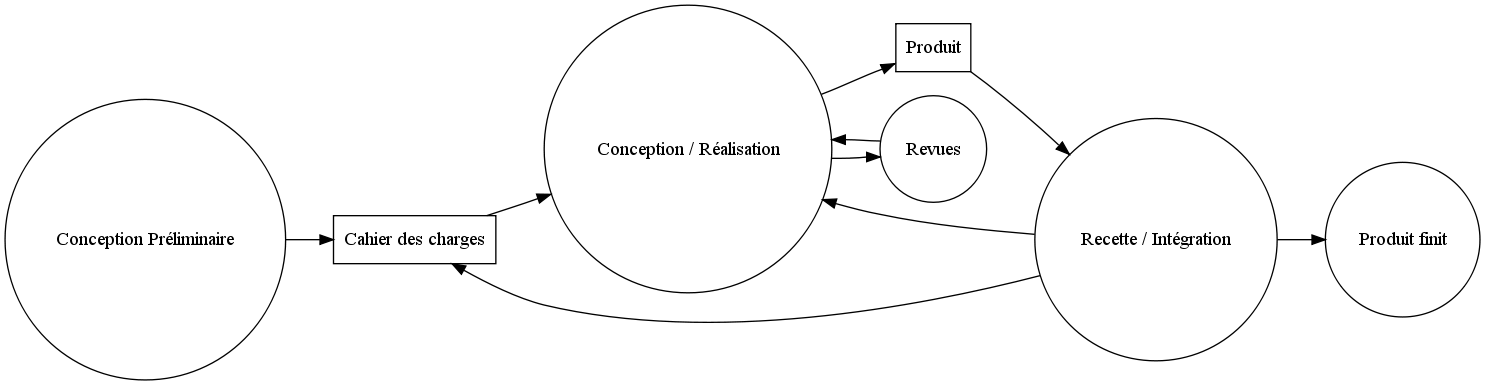
\includegraphics[width=\textwidth]{organisation.png}
\caption{Organisation du management des sous projets\label{glops}}
\end{center}
\end{figure}

    
\chapter{Décomposition en sous projets}

Ce projet étant de taille conséquente, il est impossible de confier l'ensemble de sa conception et réalisation à une unique entité. Pour cela, le projet a été séparé en différents sous projets pouvant être traités de façon indépendante par différentes entités tels que ce groupe d'étude ou différentes sociétés de service autres\ldots

\section{Critères de décomposition}

Pour cette décomposition, on utilisera plusieurs critères permettant de mettre en évidence ces sous projets. 

    \subsection{Fonctionnels} Les sous projets seront explicités en fonction des domaines fonctionnels du projet.
    \subsection{Architecturaux} En fonction des critères d'architecture matérielle.
    \subsection{Logiciels} En fonction des logiciels à développer.
    \subsection{Risque} Si une partie du projet présente des risques particuliers.

\subsection{Transversaux}

Certains projets peuvent couvrir plusieurs domaines présents, il s'agira à ce moment de projets transversaux qui doivent être traités à part.

\subsection{Charge}

Pour chaque sous projet on s'assurera que la charge sera équitablement repartie.

\section{Sous projets}

\subsection{Infrastructure matérielle}

\subsubsection{Infrastructure site distant}

Le site distant est isolé et soumis à des conditions qui peuvent parfois êtres rudes -- froids, animaux. Son infrastructure doit être la plus autonome possible, tolérante aux fautes et capable de communiquer. Ce sous projet est particulièrement critique du fait de l'éloignement du système et de son implication fonctionnelle totale.


\subsubsection{Infrastructure site central}

Le site central doit être capable de communiquer avec les différents acteurs, analyser des données et stocker celles-ci. Il sera sûrement soumis à de fortes charges et est le cœur du système de surveillance et de ce fait une pièce critique du système. Cependant sa localisation fait qu'une intervention sur celui-ci ne sera pas aussi complexe que sur les sites distants, ce qui réduit sa criticité.

\subsubsection{Télécommunications GPRS}

Ce sous projet va étudier tous les aspects liés aux communications par le protocole GPRS ainsi que les partenariats commerciaux possibles à ce niveau. 

\subsubsection{Télécommunications génériques}

Ce sous projet s'occupera de définir les infrastructures de communications entre les différents modules autre que les communications GPRS, comme les communications USB, internet\ldots

\subsection{Infrastructure logiciel}

\subsubsection{Logiciel site distant}

Le logiciel du site distant est soumis aux mêmes contraintes et besoins que l'infrastructure du même site. Cette partie logiciel est donc relativement critique.

\subsubsection{Logiciel PDA}

Il s'agit du logiciel qui sera chargé sur les assistants personnels des intervenants sur site. D'une ergonomie avancée, il permet à l'intervenant de planifier son travail et d'interagir avec les sites isolés et central. La criticité de ce logiciel n'est pas énorme du fait qu'un PDA se met à jour facilement.

\subsubsection{Logiciel site central (back end)}

Il s'agit du logiciel qui va gérer tout le système, donc très critique. Cependant la même remarque concernant le fait qu'il soit facilement accessible limite sa criticité. On notera tout de même qu'en tant que noyau du système, sa sécurité se doit d'être irréprochable.

\subsubsection{Logiciel site central (front end)}

Il s'agit principalement des interfaces que les utilisateurs auront pour accéder aux services fournis par le site central. Elles se doivent d'êtres conviviales et ergonomiques, mais ne présentent pas de gros risques.

\subsection{Projets transversaux}


\subsubsection{Communications}

Ce projet s'occupe des communications entre les différents acteurs au niveau protocoles. Il gérera la sécurité et les authentifications.

\subsubsection{Gestion de l'énergie}

Au niveau des sites distants, il faudra parfois un apport en énergie. Ce projet étudiera les sites au cas par cas pour trouver la meilleure solution possible.


\subsubsection{Formation}

Mettre en place les formations nécessaires pour tout le personnel qui aura à faire à ce système, de l'utilisateur final au technicien de maintenance.


\subsubsection{Produits dérivés}

Ce projet de surveillance de sites distants peut facilement être modifié pour être adapté à des cas similaires tels que la surveillance de personnes âgées ou de délinquants. Ce groupe de projet mettra en place les modifications nécessaires ainsi que les études commerciales associées pour vendre ces produits dérivés.


\subsubsection{Développement durable}

Dans un cadre européen, il faut prendre en compte les contraintes écologiques. Ce projet vise à mettre en place une politique durable adaptée.

\subsubsection{Normalisation}

Dans un cadre éthique et de partage de l'information, une équipe sera chargée de voir quelles sont les possibilités de normalisation du système pour permettre une réutilisation facile.






\end{document}
